\documentclass{llncs}
\usepackage{makeidx}
\usepackage{amsmath}
\usepackage{algorithm}
\usepackage[noend]{algpseudocode}
\usepackage[utf8]{inputenc}
\usepackage{cite}
\usepackage{float}
\usepackage{caption}
\usepackage[pdftex]{graphicx}
\usepackage[nottoc]{tocbibind}
\usepackage{pdfpages}
\usepackage{ragged2e}
%
\usepackage{color}
\newcommand{\PR}[1]{{\textcolor{green}{[PR: #1]}}}  % color gei
\newcommand{\DT}[1]{{\textcolor{magenta}{[DT: #1]}}}% color gei
\newcommand{\TR}[1]{{\textcolor{cyan}{[TR: #1]}}}   % color gei
\newcommand{\RK}[1]{{\textcolor{blue}{[Rk3: #1]}}}  % color gei
\newcommand{\FP}[1]{{\textcolor{orange}{[FP: #1]}}} % color gei
\newcommand{\MA}[1]{{\textcolor{red}{[MA: #1]}}}
\newcommand{\NH}[1]{{\textcolor{purple}{[NH: #1]}}} % color the rial macho

\begin{document}
\tracingall
\mainmatter

\title{Sysmic Robotics Team Description Paper}
\titlerunning{Sysmic Robotics TDP 2019}

\author{Tom\'as Rodenas, Ricardo Alfaro,  Pablo Reyes, Felipe Pinto, Maximiliano Aubel, Nicolás Hernández, Pablo Yañez, Tania Barrera, Daniel Torres, Jorge Álvarez, Damián Quiroz, Rubén González.}
%
\tocauthor{Tom\'as Rodenas, Ricardo Alfaro,  Pablo Reyes, Felipe Pinto, Maximiliano Aubel, Nicolás Hernández, Pablo Yañez, Tania Barrera, Daniel Torres, Jorge Álvarez, Damián Quiroz, Rubén González.}
%
\institute{Universidad T\'ecnica Federico Santa Mar\'ia, Valpara\'iso, Chile}

\maketitle

%%%%%%%%%%%%%%%%%%%%%%%%%%%%%%%%%%%%%%%%%%%%%%%%%%%%%%%%%%%%%%%%%%%%%%%%%%%%%%%%%%%%%%%%%%%%%%%
%                                 Abstract                                                    %
%%%%%%%%%%%%%%%%%%%%%%%%%%%%%%%%%%%%%%%%%%%%%%%%%%%%%%%%%%%%%%%%%%%%%%%%%%%%%%%%%%%%%%%%%%%%%%%
\begin{abstract}
    In this paper we briefly describe the current state of the systems implemented by our team. \PR{Comentar de forma resumida los cambios desde TDP2019 a ahora}
\end{abstract}


%%%%%%%%%%%%%%%%%%%%%%%%%%%%%%%%%%%%%%%%%%%%%%%%%%%%%%%%%%%%%%%%%%%%%%%%%%%%%%%%%%%%%%%%%%%%%%%
%                                 Mechanics                                                   %
%%%%%%%%%%%%%%%%%%%%%%%%%%%%%%%%%%%%%%%%%%%%%%%%%%%%%%%%%%%%%%%%%%%%%%%%%%%%%%%%%%%%%%%%%%%%%%%
\section{Mechanics}

\subsection{Gear-free motor to wheel connection}

\PR{Explicar de forma técnica los cambios del sistema de conexión "motor a rueda". Incorporar una imagen modelada del nuevo diseño y altura de la rueda.}

\begin{figure}[H]
    \centering
    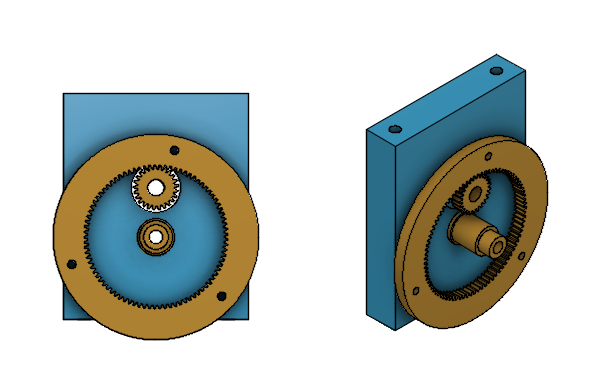
\includegraphics[scale=0.6]{Images/Engranaje.jpeg}
    \caption{Front and general view of gear system. }
    \label{fig:Wheel1}
\end{figure}

\begin{figure}[h]
    \centering
    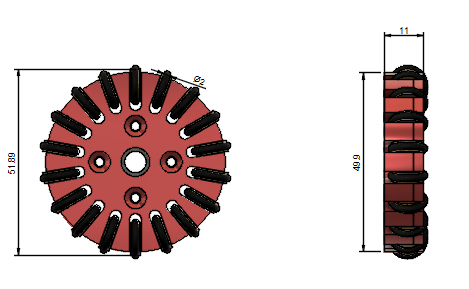
\includegraphics[scale=0.6]{Images/Wheel.jpeg}
    \caption{Front and lateral view of assembled wheel. }
    \label{fig:Wheel2}
\end{figure}

%%%%%%%%%%%%%%%%%%%%%%%%%%%%%%%%%%%%%%%%%%%%%%%%%%%%%%%%%%%%%%%%%%%%%%%%%%%%%%%%%%%%%%%%%%%%%%%
%                                 Software                                                    %
%%%%%%%%%%%%%%%%%%%%%%%%%%%%%%%%%%%%%%%%%%%%%%%%%%%%%%%%%%%%%%%%%%%%%%%%%%%%%%%%%%%%%%%%%%%%%%%
\section{Software}

\PR{En el TDP2019 se especifica que la interfaz está construida en QT, mencionar los cambios en los frameworks utilizados para el diseño de la interfaz. Si hubieron cambios en el diagrama general del sistema, también mencionarlos y rehacer la figura.}

\begin{figure}[H]
    \centering
    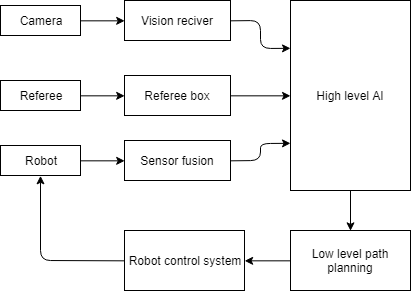
\includegraphics[scale=0.5]{gDiagram.png}
    \caption{General diagram of the system}
    \label{fig:gDiagram}
\end{figure}

\begin{figure}[h]
    \centering
    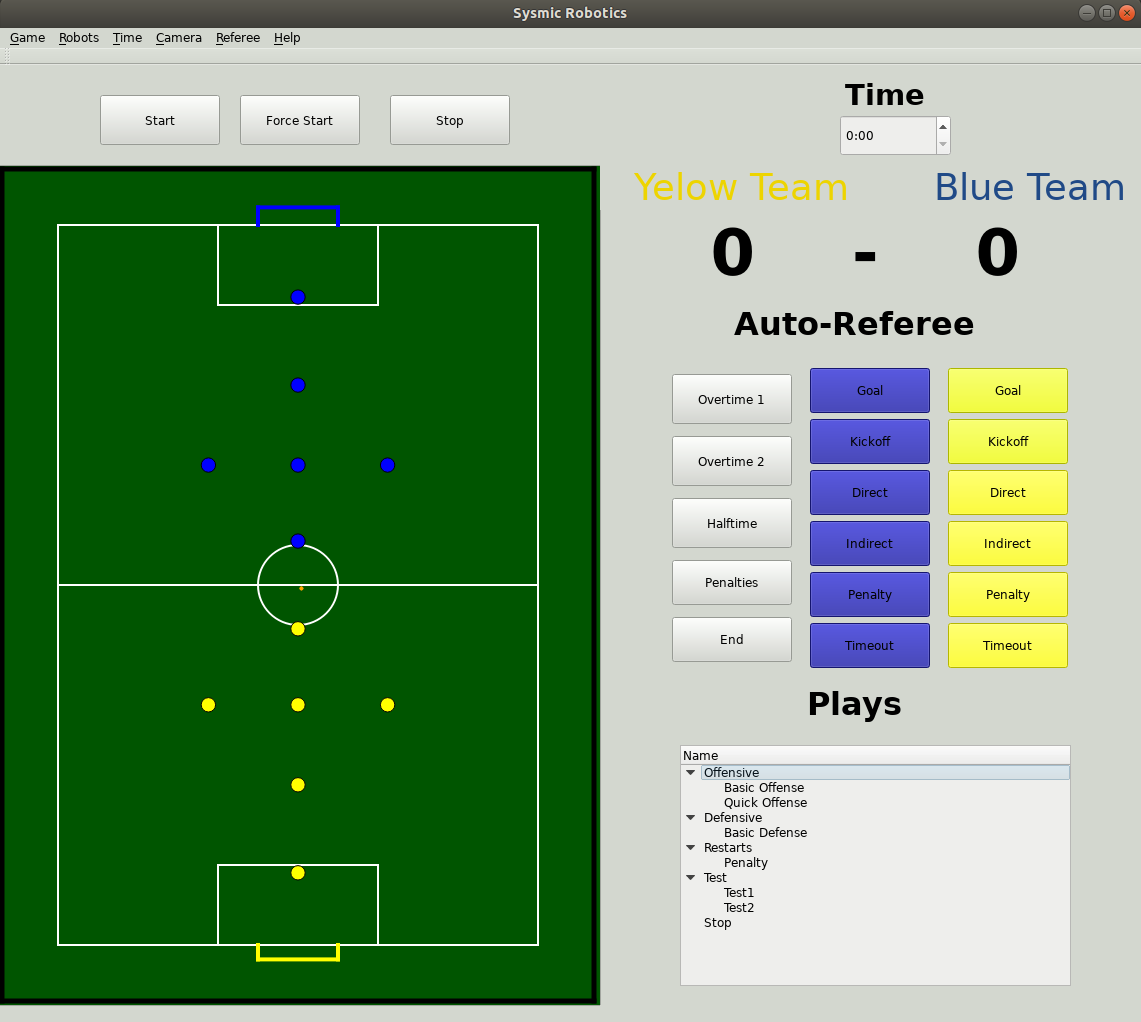
\includegraphics[scale=0.4]{GUI_F.png}
    \caption{GUI screenshot}
    \label{fig:GUI}
\end{figure}

It must be noted that this client is under construction and that we guided ourselves by the software shared by RoboJackets \cite{robojackets}. 

%%%%%%%%%%%%%%%%%%%%%%%%%%%%%%%%%%%%%%%%%%%%%%%%%%%%%%%%%%%%%%%%%%%%%%%%%%%%%%%%%%%%%%%%%%%%%%%
%                                   Sensors                                                   %
%%%%%%%%%%%%%%%%%%%%%%%%%%%%%%%%%%%%%%%%%%%%%%%%%%%%%%%%%%%%%%%%%%%%%%%%%%%%%%%%%%%%%%%%%%%%%%%
\subsection{Sensor Integration}
In the new model we integrate different kind of sensors, meaning that the robots will no longer be a peripheral to take active part in the designed AI system. The goal is to get a better estimate of the game state to enable better decision making at software level improving the game strategy, as well as at hardware level enabling a better control of the robots. Specifically we add encoders, accelerometer, gyroscope and proximity sensors.

Since the omnidirectional robots represent a nonlinear system we implement an Extended Kalman Filter  to make use of the information coming from the different kind of sensors. The main function of this algorithm is to reduce the error coming from the uncertainty present in the environment and in sensor measurement.

The encoders, accelerometer and gyroscope let us get a quicker estimate of the robot pose and velocity, since these components have a high measurement rate. However the downside of this approach is that the error propagates with the robot movement because it is relative to the robot local pose. To correct this increasing error we use the slower measurements coming from the camera taking advantage of its absolute error (since it does not depend of the robot pose and, thus, it does not propagate with it).    

Another important aspect relates to track the ball's position where we mainly use the camera information, but because of the fast nature of the game, there are significant periods of time where the robot does not know where the ball is. For that reason we implement proximity sensors to aid in the ball location when precision is needed. \PR{Se puede hacer algo al respecto de lo que está escrito?}

%%%%%%%%%%%%%%%%%%%%%%%%%%%%%%%%%%%%%%%%%%%%%%%%%%%%%%%%%%%%%%%%%%%%%%%%%%%%%%%%%%%%%%%%%%%%%%%
%                               HARDWARE
%
%%%%%%%%%%%%%%%%%%%%%%%%%%%%%%%%%%%%%%%%%%%%%%%%%%%%%%%%%%%%%%%%%%%%%%%%%%%%%%%%%%%%%%%%%%%%%%
\section{Hardware}

%%%%%%%%%%%%%%%%%%%%%%%%%%%%%%%%%%%%%%%%%%%%%%%%%%%%%%%%%%%%%%%%%%%%%%%%%%%%%%%%%%%%%%%%%%%%%%%
%                                 Kicker                                                      %
%%%%%%%%%%%%%%%%%%%%%%%%%%%%%%%%%%%%%%%%%%%%%%%%%%%%%%%%%%%%%%%%%%%%%%%%%%%%%%%%%%%%%%%%%%%%%%%
\subsection{Kicker}
%\RK{descripcion del pateador flyback}[Ruben: si existe una imagen mejor del circuito (vector), hay que actualizarla]
\PR{Mostrar la nueva placa de pateo y explicar técnicamente cómo funciona. Incorporar figura para comparar cambios.}

In the former version of our robots, the circuit of the kicking system was a Boost converter as shown in the Figure \ref{fig:old_boost}. This converter raises the voltage from the battery to 120 [V], but the main disadvantage of the circuit is the charging time, taking about 6 seconds to reach the final value. Given the dynamics and speed of the game, this charging time is excessive.

\begin{figure}[h]
    \centering
    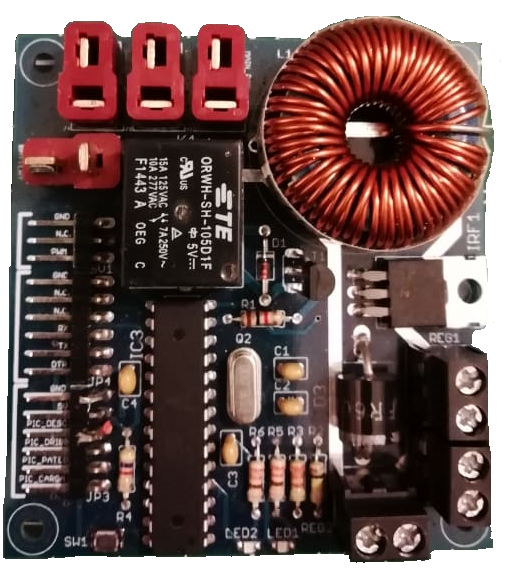
\includegraphics[width=0.5\textwidth]{Images/foto_boost.jpg}
    \caption{Old Boost circuit}
    \label{fig:old_boost}
\end{figure}

This year, the kicking system has been modified and now consists in a flyback circuit as shown in the Figure \ref{fig:kicker}. This circuit uses the Chip LT3751 which is a charger controller with regulation. The flyback circuit implements a turn ratio of 1:10 (primary:secondary) and raises the voltage from 14.8 [V] to 220 [V] on two capacitors of 1200[$\mu$F], each in less than a half second. The main advantage is that the voltage setpoint can be regulated to kick with different intensities.
%\TR{Esta imagen esta repetida en el TDP 2018. Si no hay cambios en el diseño no deberiamos ponerlo.}

\begin{figure}[h]
    \centering
    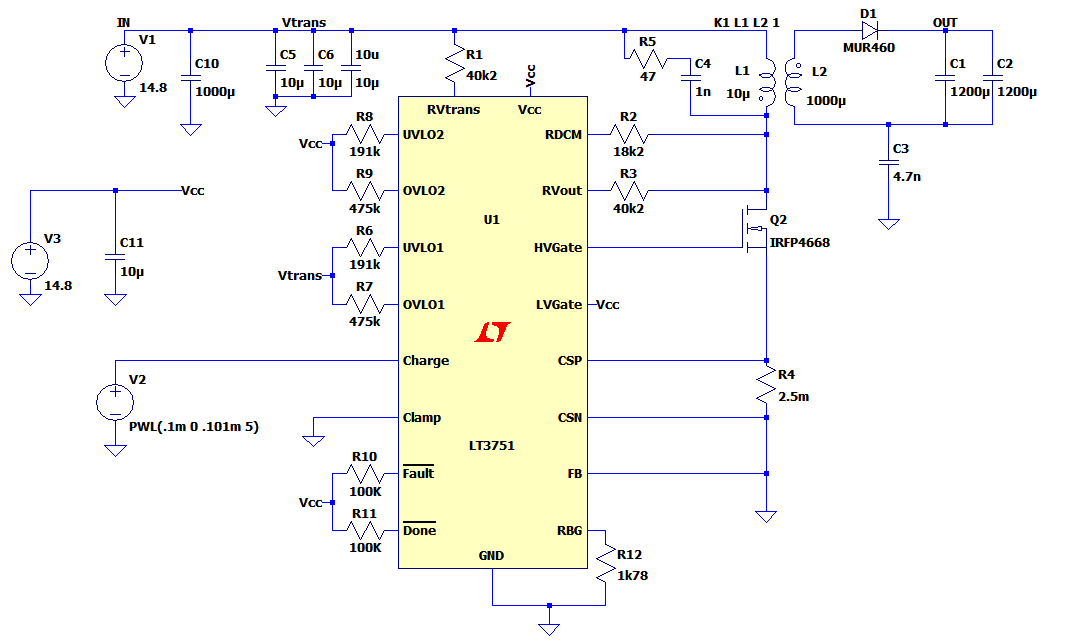
\includegraphics[scale=0.4]{Images/kicker_spice.png}
    \caption{Kicker Circuit}
    \label{fig:kicker}
\end{figure}


%%%%%%%%%%%%%%%%%%%%%%%%%%%%%%%%%%%%%%%%%%%%%%%%%%%%%%%%%%%%%%%%%%%%%%%%%%%%%%%%%%%%%%%%%%%%%%%
%                                 Bibliografy                                                 %
%%%%%%%%%%%%%%%%%%%%%%%%%%%%%%%%%%%%%%%%%%%%%%%%%%%%%%%%%%%%%%%%%%%%%%%%%%%%%%%%%%%%%%%%%%%%%%%
\bibliographystyle{plain}
{
    \renewcommand{\clearpage}{} 
    \bibliography{biblio.bib}
}



%%%%%%%%%%%%%%%%%%%%%%%%%%%%%%%%%%%%%%%%%%%%%%%%%%%%%%%%%%%%%%%%%%%%%%%%%%%%%%%%%%%%%%%%%%%%%%%
%                             Acknowledgments                                                 %
%%%%%%%%%%%%%%%%%%%%%%%%%%%%%%%%%%%%%%%%%%%%%%%%%%%%%%%%%%%%%%%%%%%%%%%%%%%%%%%%%%%%%%%%%%%%%%%
\section*{Acknowledgments}

Sysmic Robotics would like to acknowledge the previous team members that helped us to get here and to all the people that support and help us in any way. We could not have made it alone.

% that's all folks
\end{document}